\documentclass[sigconf]{acmart}
\usepackage{booktabs} % For formal tables
\usepackage{subcaption}
\usepackage{mathtools}
\usepackage{amsmath}
\usepackage{pbox}
\usepackage{flushend}

\usepackage{xcolor}
\usepackage{colortbl}


\setcopyright{rightsretained}

% DOI
%\acmDOI{10.475/123_4}

% ISBN
% \acmISBN{123-4567-24-567/08/06}

%Conference
%\copyrightyear{2017}
%\acmYear{2017}
%\setcopyright{acmlicensed}     
%\acmConference{ACM-BCB'17}{}{August 20-23, 2017, Boston, MA, USA.} 
%\acmPrice{15.00} 
%\acmDOI{https://doi.org/10.1145/3107411.3116251}
% check your pdf to see if "http://" is duplicated. 
%\acmISBN{978-1-4503-4722-8/17/08}

\settopmatter{printacmref=false, printfolios=false}

\fancyhead{}

\begin{document}
\title{ProMuteHT 2.0 : A High Throughput Compute Pipeline for Generating
  Protein Mutants \textit{in silico}}

\author{Katie Hursh}
\affiliation{%
  \institution{Western Washington University}
  \streetaddress{516 High Street}
  \city{Bellingham} 
  \state{WA} 
  \postcode{98225}
}
\email{hurshk@wwu.edu}

\author{Filip Jagodzinski}
\affiliation{%
  \institution{Western Washington University}
  \streetaddress{516 High Street}
  \city{Bellingham} 
  \state{WA} 
  \postcode{98225}
}
\email{filip.jagodzinski@wwu.edu}

\renewcommand{\shorttitle}{ProMuteHT 2.0}


\begin{abstract}
Understanding how the structure of a protein changes with an amino acid substitution is vital for both the advancement of medicine and protein docking studies. In vitro experiments are both time and cost prohibitive, and may require months of wet lab work to mutate and determine the structure of the mutant via X-ray crystallography. In this work we are developing a program for generating in silico protein mutants. Our software ProMuteHT provides a high-throughput platform to generate a large number of mutants with a simple command line interface. ProMuteHT is different from other in silico approaches in that it relies on the structure of the protein as a seed for generating a mutant, rather than using complex and expensive energy calculations.  We show improvement in run times over FoldX and the previous version of the program while still keeping a reasonable level of quality of the results.
\end{abstract}

%
% The code below should be generated by the tool at
% http://dl.acm.org/ccs.cfm
% Please copy and paste the code instead of the example below. 
%
\begin{CCSXML}
<ccs2012>
<concept>
<concept_id>10010405.10010444.10010087.10010098</concept_id>
<concept_desc>Applied computing~Molecular structural biology</concept_desc>
<concept_significance>500</concept_significance>
</concept>
<concept>
<concept_id>10010405.10010444.10010450</concept_id>
<concept_desc>Applied computing~Bioinformatics</concept_desc>
<concept_significance>300</concept_significance>
</concept>
</ccs2012>
\end{CCSXML}

\ccsdesc[500]{Applied computing~Molecular structural biology}
\ccsdesc[300]{Applied computing~Bioinformatics}

\keywords{Mutagenesis; in silico; Modeling; Protein Structure}

\maketitle

\section{Introduction}
The study of the effects of mutations is important for the advancement of research in the areas of disease and drugs.  Disease such as Sickle Cell, Huntington's and cancer are all the result of mutations.  While those type of mutations are detrimental, others can be used in the generation of medications to help fight these and other ailments.

One way of studying the results of mutations is to perform mutagenesis on physical proteins in wetlabs.  Once the mutation is performed, X-ray crystallography is used to determine the final structure.  These experiments take a prohibitive amount of time and money to perform, and not all structures are measurable through crystallography.  These experiments are very impractical to attempt at random, and thus very few mutagenesis experiments have been performed.

Using computers to estimate the effects of these mutations \textit{in silico} can provide an answer to the problems of both the speed and expense of the \textit{in vitro} experiments.  The \textit{in silico} mutation results can be evaluated to shorten the list of mutations that should be performed in wetlabs, saving a huge amount of time and money.

%1~\cite{reva2011} 2~\cite{mishra2012} 
%3~\cite{schellman1987} 
%4 ~\cite{dunbrack1994,wodak1978, ponder1987} 5~\cite{gilis1997, lee1991} 6~\cite{topham1997, worth2011, brender2015} 7~\cite{cheng2006, akbal2013} 8~\cite{jia2015, li2012,bromberg2008,hecht2015}

\section{Related Work}
In this section, we will discuss a number of the other programs that exist to perform \textit{in silico} mutant generation.  These programs require a significant amount of human intervention or costly energy calculations in order to perform the desired mutation.  Early versions of these programs modified energy and structure parameters of simulated proteins, yet did not generate or modify structure files~\cite{you2002}.  More recent programs, such as Swiss PDB Viewer~\cite{guex1997}, PyMol~\cite{delano2002}, and FoldX~\cite{schymkowitz2005} provide a richer interface and generate the final structure file after the desired mutations.

Swiss PDB Viewer provides a graphical user interface and scripting system to allow for mutations and visualizations.  The documentation and support for the program is limited and will only work on Windows and Mac operating systems with no command line interface, which makes it difficult to incorporate into a larger automation pipeline.

PyMol provides a more powerful user interface and scripting system along with command line invocations.  The program guides the user through the mutation process using a visual guide and rotamer library to increase the quality of the resulting mutation.  It is however limited in that mutations can only be performed manually through the user interface.

The FoldX software suite also provides a user interface and command invocations, but it also allows for mutations to be performed from the command line.  This process requires that all of the desired mutations be listed in a configuration file that is then fed to the program.  The mutations in FoldX are based on an empirical energy field to determine the results of a mutation.  This involves calculating a linear combination of nine empirical energy terms, such as hydrogen bond and steric clash energies, for the protein for each mutation that needs to be performed.

The previous version of ProMuteHT~\cite{andersson2017} provided an entirely command line-based invocation. This program allowed for a highly scriptable process with very little human interaction necessary. The mutation process for this program is summarized in Figure~\ref{proMute1Pipeline}.  ProMuteHT showed a significant increase in speed over other work such as FoldX without losing an impractical amount of quality in the process.

In addition to the programs listed, there are a number of other methods used to complement the work performed in a wetlab.  Some studies reason about the effects of changing side-chain conformations~\cite{dunbrack1994,wodak1978, ponder1987}. Other methods have taken into account energy functions or database-derived potentials~\cite{gilis1997, lee1991} or use large datasets of closely related proteins~\cite{topham1997, worth2011, brender2015}.  A variety of machine learning approaches have also been used~\cite{cheng2006,akbal2013,jia2015,li2012,bromberg2008,hecht2015}.  Many of these methods do not generate a structure file that can be used in other programs however.

%1~\cite{you2002} 2~\cite{delano2002} 3~\cite{guex1997} 4~\cite{schymkowitz2005}

\begin{figure}[t]
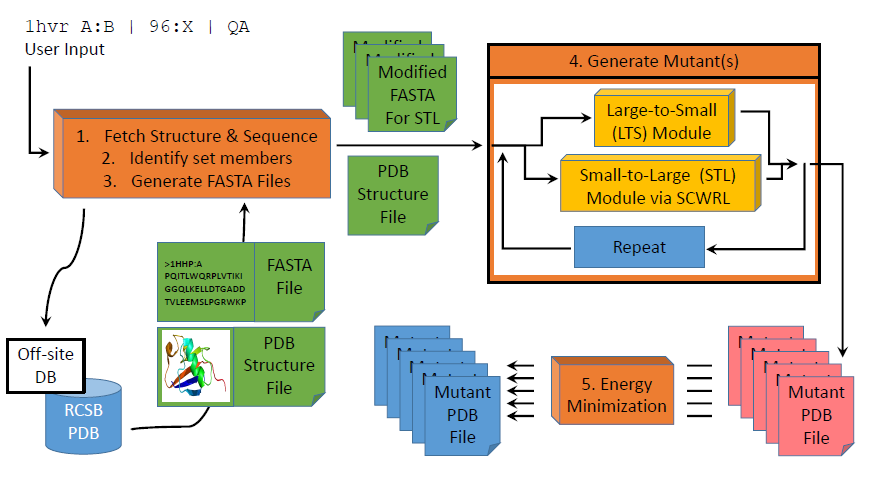
\includegraphics[width=0.95\columnwidth]{Figures/proMute1.png}
\caption{ProMuteHT 1.0 fetches a protein structure and its FASTA file from the PDB (1), enumerates a mutant list per the user's input parameters (2), processes the FASTA file as needed by SCWRL~\cite{krivov2009} when a small-to-large mutation is required (3), and iteratively generates mutant files (4) which then are energy minimized (5).}
\label{proMute1Pipeline}
\end{figure}

\section{Motivation}
Due to the issues discussed earlier with physical experiments, there needs to be a way to generate \textit{in silico} mutations to estimate the effect of mutations on any given protein.  Due to the huge number of possible mutations of a protein, manual intervention by humans, even for \textit{in silico} mutations, becomes prohibitively expensive and error prone as well.  Even a relatively small protein like 1LZ1 has millions of different possible mutations and mutation combinations.

While some programs such as FoldX allow for automation of the mutation process, the expensive energy and force calculations that are performed with every mutation causes a computational overhead that makes a large number of mutations impractical.  

ProMuteHT 1.0 addressed the time issue by taking advantage of the structure of the proteins to generate the mutant in order to rely on energy calculations as little as possible.  The original version is limited in the types of mutations that it can perform however. For example, it cannot perform mutations across multiple chains in the same protein and it cannot handle mutations on proteins where the PDB structure file is missing residues.

ProMuteHT 2.0 improves on the speed and usability of ProMuteHT 1.0 with the following advancements:
\begin{enumerate}
\item Reduce the amount of file input and output
\item Reduce the number of energy calculations further by only running energy minimization under certain conditions
\item Rewrite the program in C++ to increase speed, ease of use and portability
\item Change the handling of multi-chain proteins to increase accuracy and allow more mutations to be performed
\end{enumerate}

%1~\cite{gray2003} 2~\cite{ballester2010}

\section{Methods -- Compute Pipeline}
With the project goals in mind, we restructured the process in which the mutation occurs.  See Figure~\ref{proMute2Pipeline} for a summary of this process.

\begin{figure}[b]
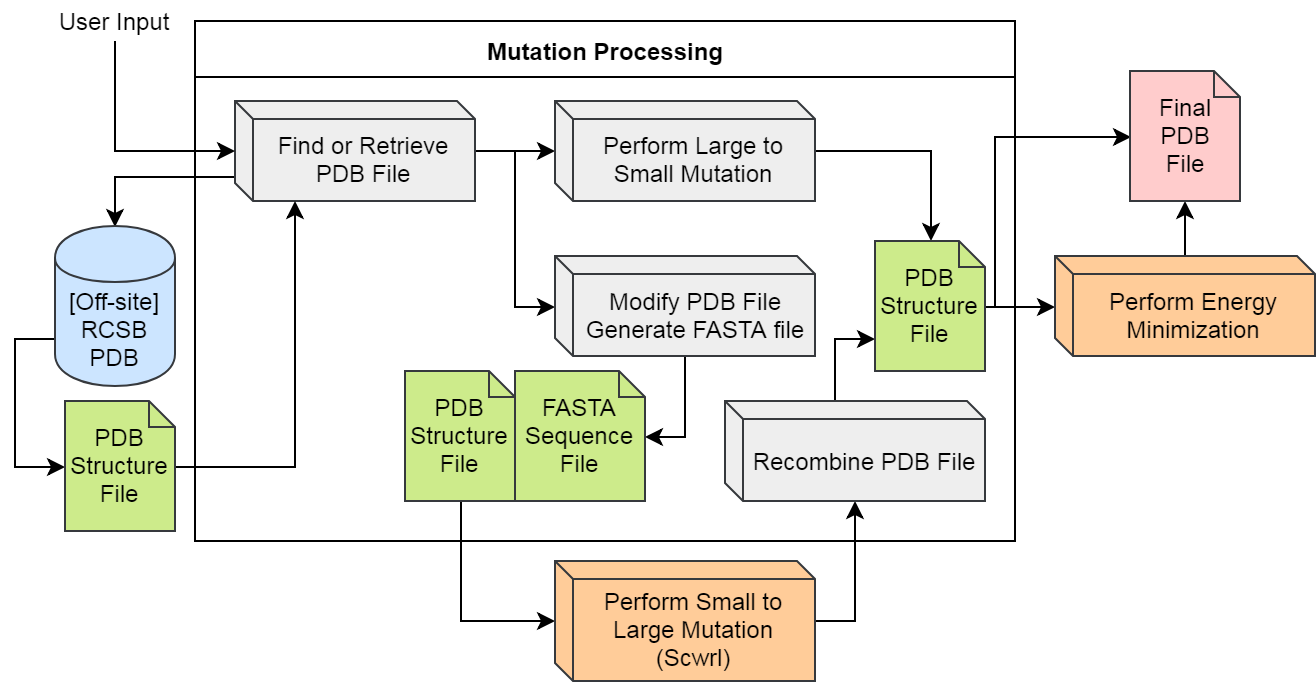
\includegraphics[width=0.95\columnwidth]{Figures/proMute2.png}
\caption{ProMuteHT 2.0 retrieves the protein structure from PDB only if needed.  If the mutation is large-to-small, the mutation is performed in-program, otherwise a PDB and FASTA file are generated for SCWRL.  A final structure file is created and run through Energy Minimization if necessary.}
\label{proMute2Pipeline}
\end{figure}

\subsection{Parameter Input}
The two command line input formats accepted by ProMuteHT 2.0 are intended to be as simple as possible to increase accessibility and ease of scripting.  The first format defines a single mutation and follows the general structure of:

$$\texttt{Source chain residue mutant [EM]}$$ 

\noindent where \texttt{Source} is the 4 character alphanumeric structure ID from the Protein Data Bank~\cite{bernstein1977}, or the file name without the extension of a previously generated mutation structure file. \texttt{chain} specifies which chain the mutation should be performed on.  \texttt{residue} denotes the number of the specific residue that will be mutated. \texttt{mutant} is the single character representation of the amino acid that the residue will be mutated to.  \texttt{EM} is an optional argument that allows the user to choose if they would like to force energy minimization (em) or skip energy minimization (no).  If the \texttt{EM} argument is not present, whether or not energy minimization will be run is determined by the program.  See Section 4.3 for more details on this decision process.

The second input format allows for users to use the format set up for the original version of ProMuteHT~\cite{andersson2017}.  This follows the format of:

$$\texttt{PDBID chain$_{s}$:chain$_{e}$ res$_{s}$:res$_{e}$,res$_n$${\{^X\}}$ subs}$$ 

\noindent where \texttt{PDBID} is the 4 character alphanumeric structure ID from the Protein Data Bank~\cite{bernstein1977}, \texttt{chain$_{s}$} and \texttt{chain$_{e}$} specify a range of chains to apply each mutation to, \texttt{res$_{s}$} and \texttt{res$_{e}$} specify a range of residues to apply the mutations to, \texttt{res$_{n}$} are individual residues, or additional ranges of residues, delimited by commas. 

%~\ref{proMutePipeline}
%1~\cite{bernstein1977}

%\subsection{Generating Mutants} 1~\cite{krivov2009} 2~\cite{bower1997}

\begin{figure}[t]
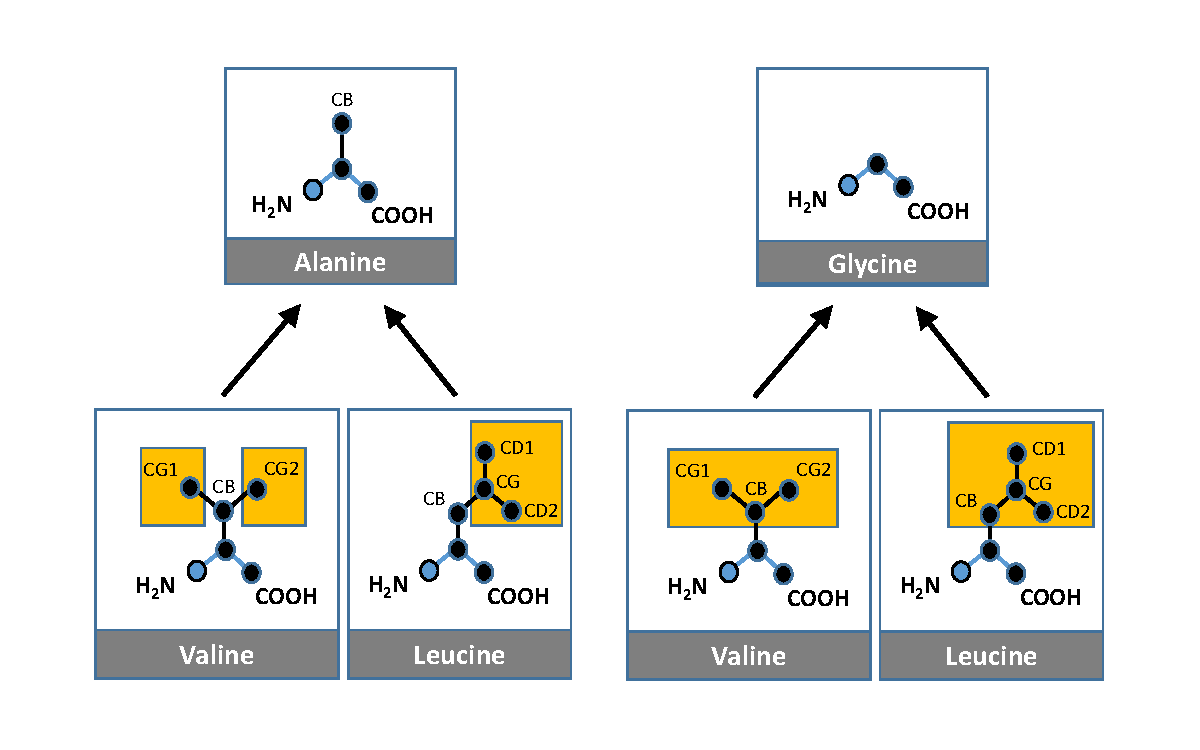
\includegraphics[width=0.85\columnwidth]{Figures/lts.pdf}
\caption{Large-to-small (LTS) mutations in ProMuteHT do not require energetics calculations. The \textit{in silico} mutation involves retaining only the atoms of the target, smaller, residue. To mutate Valine or Leucine to Alanine, we remove the carbon atoms at the $\gamma$ and $\delta$ positions (yellow boxes).}
\label{LTS}
\end{figure}

\subsection{Mutating Single Chain Proteins}
When mutating single chain proteins, the mutation process is either handled inside of ProMuteHT or it is passed to SCWRL to complete. ProMuteHT handles all mutations internally if the mutation is Large-to-Small and the target amino acid is either a Glycine, Alanine, or Serine.  For all other mutations, the program creates a sequence file from the input PDB and sends to SCWRL to perform the mutation.

For those mutations that are handled internally, the mutations are performed by directly removing all atoms from the source amino acid that would not be in the target amino acid. The atoms that remain for the mutated residue are updated to reflect the new type of residue.  All other residues in the protein remain unchanged.  No positions are updated during this process nor any expensive calculations performed.

SCWRL performs mutations on the proteins by using a rotamer library~\cite{bower1997} based on kernel density estimates to predict the effect on side chain conformations.  It relies on a number of metrics such as van der Waal interaction potential and a hydrogen bonding function.  While this program is fast, it still requires calculations that slow down 

\subsection{Mutating Multiple Chain Proteins}
\begin{figure}[h]
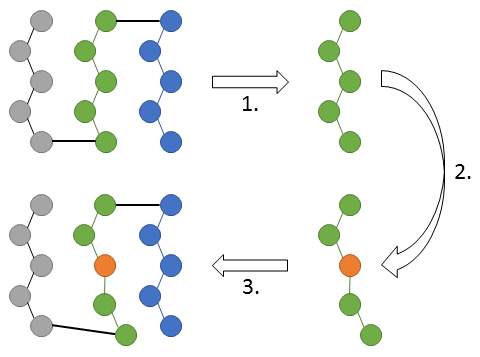
\includegraphics[width=0.85\columnwidth]{Figures/MultiChain.png}
\caption{The process of performing a mutation on a multi-chain protein. The chain is separated from the other chains (1), the mutation is performed (2), then the mutated chain is inserted back into the original spot for that chain (3)}
\label{multi}
\end{figure}

For proteins that have multiple chains, the criteria for being handled internally in ProMuteHT or sending to SCWRL is the same as the single chain proteins.  If the mutation is handled internally, there is no difference from the single chain process.  If the mutation is handled by SCWRL, the chain that contains the residue being mutated is separated from the other chains in the protein.  The sequence and structure files given to SCWRL are created with only the separated chain.  The program then reads the structure file created by SCWRL and replaces the old version of that chain with the new mutated chain.  No other chains are modified during this process.

\subsection{Energy Minimization}
Energy Minimization is handled by the NAMD~\cite{phillips2005} software using 200 steps.

Due to the expensive calculations required to perform Energy Minimization, we take advantage of the structural properties of a protein to determine if the extra calculations are worth the time cost. First we take a look at the Solvent Accessible Surface Area (SASA) of the residue that is being mutated.  The higher the SASA, the fewer residues will be surrounding or neighboring that residue.  This means that a mutating a highly accessible residue would be much less likely to have any significant effect on the energy balance of the protein as a whole.  If the SASA is above a certain threshold, in this case 50, energy minimization will not be performed.  

If below the threshold, the program will then check if the mutation is a Large-to-Small mutation.  If the mutation is not Large-to-Small, this means that atoms are being added to the side chain or being manipulated to create a different amino acid.  Due to these additions or shifts, atoms could become too close to other atoms, causing a steric clash.  In this case, the program will run Energy Minimization to resolve any clashes.  If the mutation is Large-to-Small, the are no new atoms being introduced, so there is a tiny chance of any clash occurring, thus energy minimization is not run.

%1~\cite{phillips2005}

\section{Results}
Table~\ref{summary} is a summary of all of the \textit{in silico} experiments that were run.  In order to assess the results of these experiments, we tallied runtimes of ProMuteHT 2.0 versus FoldX and ProMuteHT 1.0 as well as using the root mean squared difference (RMSD) of the results of the experiments versus the wetlab results stored in the RCSB Protein Data Bank (PDB).  All times were measured using the \textit{real} result of the Linux \textit{time} command.

\begin{figure}[h]
	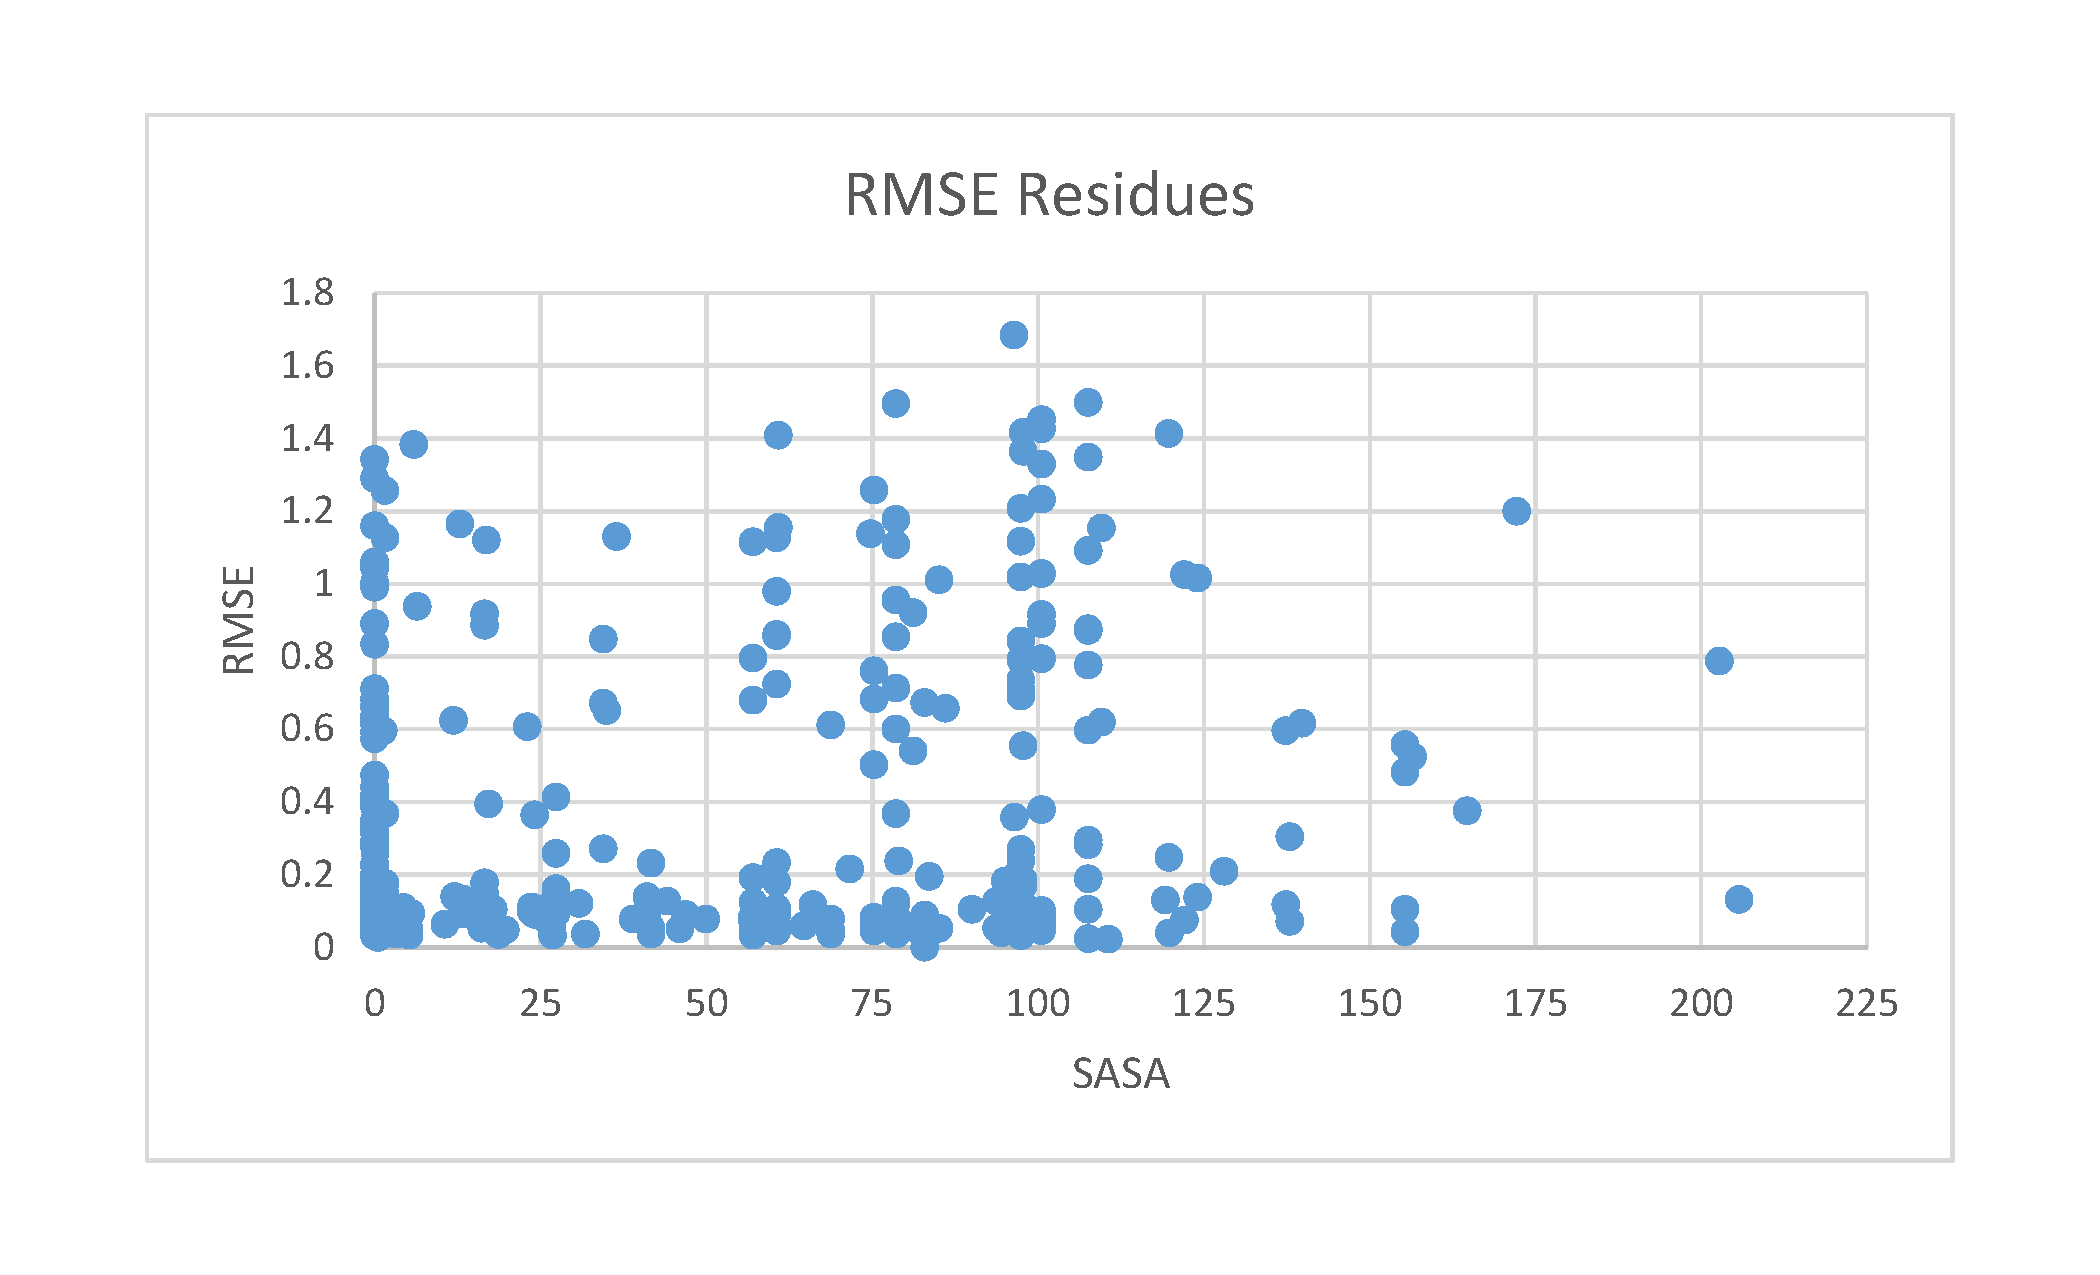
\includegraphics[width=1.1\linewidth]{Figures/Results.pdf}
	\caption{Scatter Plot of the RMSD for all tested mutations against the SASA of the last mutated residue}
	\label{result}
\end{figure}
\begin{table}[h]
	\caption{Summary of RMSD for all experiments }
	\label{summary}
	\centering
	\begin{tabular}{|c|c|c|c|c|c|c|} \hline
		\rowcolor{lightgray}Multi &  &  &  &  & \multicolumn{2}{c|}{Ave. RMSD} \\
		\rowcolor{lightgray}Mut. & SASA & Size & EM? & Count & All & Residues \\ \hline
		No & $<$ 50 & L$\rightarrow$ S & No & 98 & 0.4236 & 0.2153 \\ \hline
		No & $<$ 50 & S$\rightarrow$L & Yes & 53 & 0.4450 & 0.5044 \\ \hline
		No & $\ge$ 50 & L$\rightarrow$S & No & 79 & 0.2083 & 0.3484 \\ \hline
		No & $\ge$ 50 & S$\rightarrow$L & No & 70 & 0.9609 & 0.6397 \\ \hline
		Yes & $<$ 50 & L$\rightarrow$S & No & 17 & 0.2524 & 0.2474 \\ \hline
		Yes & $<$ 50 & S$\rightarrow$L & Yes & 8 & 0.4445 & 0.4544 \\ \hline
		Yes & $\ge$ 50 & L$\rightarrow$S & No & 10 & 1.2160 & 0.4298 \\ \hline
	\end{tabular}
\end{table}

The RMSDs of all proteins where both the Wild Type and the Mutated protein are stored in PDB and the chain mutated is discernible is stored in Table~\ref{AllResults}.

\subsection{ProMuteHT 2.0: speed improvements}
In Table~\ref{tab:benchmarking} we show 4 invocations compared between the two versions of ProMuteHT using 13, 171, 342, and 418 mutants.

\begin{table}[h]
	\caption{Run Times for sample invocations of ProMuteHT.  The columns for the run-times correspond to results for the previous version (1.0) and the current version (2.0) of ProMuteHT.}
	\label{tab:benchmarking} 
	\centering
	\begin{tabular}{|c|c|c|c|c|} \hline
		\rowcolor{lightgray} &  &  & \multicolumn{2}{c|}{run-time (s)}\\
		\rowcolor{lightgray}Invocation & \# Res & \# Muts & 1.0 & 2.0\\ \hline
		$\texttt{1hhp A:A 3,7,10:20 G}$ & 99 & 13 & 21.9 & 0.6 \\ \hline
		$\texttt{1crn A:A 12:30 pol}$ & 46 & 171 & 220 & 106 \\ \hline
		$\texttt{1pef A:A X:X X}$ & 18 & 342 & 407 & 45 \\ \hline
		$\texttt{1hvr A:B 20:30 X}$ & 198 & 418 & 586 & 954\\ \hline
	\end{tabular}
\end{table}

\subsection{ProMuteHT v.s. FoldX: Speed}
In Table~\ref{tab:foldxcompare}, we compare two invocations of FoldX, ProMuteHT 1.0 and ProMuteHT 2.0.

For the FoldX invocations, the mutation configuration file was created before the timing of the mutation.  For larger numbers of mutations, this configuration file creation would take a prohibitive amount of time, or would require that another program be created in order to generate them.

Both versions of ProMuteHT show a decrease in total runtime over FoldX.  We suspect that this decrease is due to the expensive calculation that FoldX performs on every mutation.

\begin{table}[h]
	\caption{FoldX vs ProMuteHT run times for \textit{in silico} generating two sets of mutants with 5 and 18 structures each. The columns for the run-times correspond to results for FoldX, the previous version (1.0) and the current version (2.0) of ProMuteHT.}
	\label{tab:foldxcompare} 
	\centering
	\begin{tabular}{|c|c|p{2.8cm}|c|c|c|} \hline
		\rowcolor{lightgray}& & \multicolumn{1}{c|}{Mutants} & \multicolumn{3}{c|}{Run-Times (s)}\\
		\cline{4-5}
		\rowcolor{lightgray} PDB & \# Muts & (comma delimited) & FoldX & 1.0 & 2.0\\ \hline
		1hhp& 6 & L19G and K20A, L19G and E21A, L19G and E22A, L19G and L23A, L19G and L24A, L19G and D25A & 82.5 & 12.3 & 0.8 \\ \hline
		1pef& 18 & E1G, Q2G, L3G, L4G, K5G, A6G, L7G, E8G, F9G, L10G, L11G, K12G, E13G, L14G, L15G, E16G, K17G, L18G & 66.5 & 32 & 0.5 \\ \hline
	\end{tabular}
\end{table}

\subsection{ProMute v.s. FoldX: Quality}
In order to measure the quality of each of the tested programs, we selected 19 proteins pairs where both the wild type protein and the mutagenesis experiment result are both available in the PDB.  In this case, 8 of the pairs has 1LZ1 as the wild type protein and 11 had 2LZM as the wild type protein.  For each of these protein pairs, we took the wild type and performed the mutation in each of the three programs.  The results of each of the programs were then compared against the PDB's mutant file to calculate the RMSD when aligning the entire protein (RMSD All) or aligning only on the residues that were mutated (RMSD Res). The results are available in Table~\ref{tab:RSMDResults}.

\begin{table}[h]
	\centering
	\caption{The quality of variants output by ProMuteHT was assessed by comparing \textit{in silico} generated mutants with mutant structures from the PDB with equivalent mutations. Res=residue in the polypeptide chain, AA=Amino Acid for the wild type and Mutant for the indicated Res, and ASA=Accessible Surface Area. RMSD=Root Mean Squared Deviation between the actual (from PDB) and \textit{in silico} generated mutants. These were calculated for the generated mutants from FoldX (FX), ProMuteHT 1.0 (1.0) and ProMuteHT 2.0 (2.0)}
	\label{tab:RSMDResults} 
	\setlength\tabcolsep{4pt}
	\resizebox{\columnwidth}{!}{%
	\begin{tabular}{|c|c c c|c c|c|c|c|c|c|c|} \hline
		\rowcolor{lightgray} \multicolumn{4}{|c|}{WT Structure} & \multicolumn{2}{c|}{Mutant} & \multicolumn{3}{c}{RMSD all} & \multicolumn{3}{c}{RMSD res} \\
		\cline{1-10}
		\rowcolor{lightgray}PDB & res & AA & ASA & AA & PDB & FX & 1.0 & 2.0 & FX & 1.0 & 2.0\\ \hline
		1lz1 & 2 & V & 0 & R & 1gfg & 0.22 & 0.25 & 0.25 & 0.85 & 0.77 & 0.78 \\
		1lz1 & 110 & V & 60.1 & Y & 1gft & 0.27 &  0.31 & 0.32 & 0.03 & 1.31 & 1.33 \\
		1lz1 & 110 & V & 60.1 & D & 1gfu & 0.22 & 0.26 & 0.27 & 0.91 & 1.10 & 1.43 \\
		1lz1 & 56 & I & 0.3 & T & 1oua & 0.22 & 0.41 & 0.23 & 0.08 & 0.15 & 0.15 \\
		1lz1 & 54 & Y & 8.1 & F & 1wqq & 0.21 & 0.22 & 0.23 & 0.77 & 0.06 & 0.06 \\
		1lz1 & 56 & I & 0.3 & V & 2bqd & 0.23 & 0.26 & 0.26 & 0.11 & 0.10 & 0.10 \\
		1lz1 & 56 & I & 0.3 & A & 2hec & 0.21 & 0.21 & 0.21 & 0.04 & 0.04 & 0.05 \\
		1lz1 & 59 & I & 1.6 & G & 2hee & 0.22 & 0.22 & 0.23 & 0.03 & 0.03 & 0.03 \\
		2lzm & 157 & T & 41.8 & H & 1l09 & 0.08 & 0.11 & 0.11 & 0.85 & 1.12 & 1.13 \\
		2lzm & 99 & L & 0 & I & 1l92 & 0.13 & 0.15 & 0.32 & 0.26 & 0.07 & 0.05 \\
		2lzm & 99 & L & 0 & M & 1l93 & 0.13 & 0.15 & 0.15 & 1.1 & 1.06 & 1.06 \\
		2lzm & 3 & I & 10.7 & P & 1l96 & 0.21 & 0.24 & 0.25 & 0.21 & 0.17 & 0.18 \\
		2lzm & 105 & Q & 32.5 & E & 1l98 & 0.22 & 0.25 & 0.25 & 0.21 & 0.14 & 0.14 \\
		2lzm & 42 & A & 0 & S & 206l & 0.15 & 0.15 & 0.32 & 0.04 & 0.03 & 0.57 \\
		2lzm & 44 & S & 57.5 & W & 216l & 0.9 & 0.96 & 0.95 & 0.01 & 0.10 & 1.18 \\
		2lzm & 6 & M & 0 & L & 230l & 0.2 & 0.22 & 0.34 & 0.68 & 0.35 & 0.40 \\
		2lzm & 120 & M & 16.4 & K & 232l & 0.19 & 0.22 & 0.32 & 0.21 & 0.17 & 0.12 \\
		2lzm & 149 & V & 0 & C & 237l & 0.17 & 0.19 & 0.17 & 0.05 & 0.04 & 0.05 \\
		2rn2 & 48 & E & 10.8 & Q & 1rdb & 0.19 & 0.23 & 0.32 & 0.18 & 0.17 & 0.14 \\
		\hline
	\end{tabular}}
\end{table}

\section{Conclusions}
We have developed ProMuteHT 2.0 to build on the features of ProMuteHT 1.0  and to further increase the efficiency.  With these goals, we were able to decrease the run times in almost all cases by a significant margin.  We were able to reduce the number of file reads and writes by performing majority of the calculations and processes in memory.  We were able to further reduce the average number of energy calculations by choosing whether or not energy minimization run on a per-mutation basis rather than always running it.

With this increase in efficiency, we still managed to keep an acceptable quality compared to ProMuteHT 1.0. In some cases, we even saw an increase in the quality over the original version.

There are still limitations with this new version.  Currently, the program cannot handle multiple mutations within the same run of the program.  This causes an inefficiency by requiring any outputted file to be read by the program again to perform any further mutations on the same file.  This also causes the last mutation in a sequence to determine if Energy Minimization should be run, rather than evaluating the entire chain of mutations for any mutations that meet the criteria.

With the next version of the program, a further update to the command line arguments would go a long way to fixing the issues listed above.  If multiple mutations are handled by a single run of the program, the protein structure could be copied and modified in memory, further reducing the need for file access.  This would also allow all mutations that need to be evaluated by SCWRL for a given mutation chain to be handled at one time, rather than through multiple invocations. Another possible way to increase efficiency further would be to introduce parallel processing of multiple separate mutations to a given source protein.

\bibliographystyle{ACM-Reference-Format}
\bibliography{proMute2} 

\clearpage
\begin{table*}[h]
	\tiny
	\caption{RMSD results of all experiments run through ProMuteHT 2.0 vs. the corresponding wet lab experiment stored in the PDB.}
	\label{AllResults}
	\resizebox{\textwidth}{!}{%
	\begin{tabular}{|c|c|p{2.8cm}|c|p{2.8cm}|c|c|c|c|c|} \hline
		\rowcolor{lightgray}  &  &  &  &  &  &  &  & \multicolumn{2}{c|}{RMSD} \\
		\rowcolor{lightgray} Source & Destination & Mutations & Chains & SASA & Mutator & L $\rightarrow$ S? & EM? & All & Residues \\ \hline
		1AMQ & 1QIR & C 191 Y & Single & 1.55 & Scwrl & No & Yes & 0.669 & 1.126 \\ \hline
		1AMQ & 1QIS & C 191 F & Single & 1.55 & Scwrl & No & Yes & 0.642 & 0.368 \\ \hline
		1AMQ & 1QIT & C 191 W & Single & 1.55 & Scwrl & No & Yes & 0.677 & 1.257 \\ \hline
		1AMQ & 5EAA & C 191 S & Single & 1.55 & ProMute & No & Yes & 0.413 & 0.176 \\ \hline
		%1ARR & 1MYK & P 8 L & Multi & 35.22 & Scwrl & No & Yes & 0.772 & 6.704 \\ \hline
		1BPI & 1AAL & C 30 V, C 51 A & Single & 17.36, 0 & ProMute & Yes & No & 0.399 & 0.473 \\ \hline
		1BPI & 1BPT & Y 23 A & Single & 0.78 & ProMute & Yes & No & 0.318 & 0.094 \\ \hline
		1BPI & 1BTI & F 22 A & Single & 16.16 & ProMute & Yes & No & 0.298 & 0.052 \\ \hline
		1BPI & 1FAN & F 45 A & Single & 13.35 & ProMute & Yes & No & 0.28 & 0.092 \\ \hline
		1BPI & 1NAG & N 43 G & Single & 0 & ProMute & Yes & No & 0.366 & 0.038 \\ \hline
		1BPI & 7PTI & C 30 A, C 51 A & Single & 17.36, 0 & ProMute & Yes & No & 0.307 & 0.224 \\ \hline
		1BPI & 8PTI & Y 35 G & Single & 11.9 & ProMute & Yes & No & 0.853 & 0.624 \\ \hline
		1CEY & 1E6K & D 12 A & Single & 0 & ProMute & Yes & No & 1.664 & 0.176 \\ \hline
		1CEY & 1E6L & D 13 A & Single & 46.85 & ProMute & Yes & No & 1.411 & 0.09 \\ \hline
		1CEY & 1E6M & D 57 A & Single & 0 & ProMute & Yes & No & 1.307 & 0.387 \\ \hline
		1IOB & 1HIB & T 9 G & Single & 1.2 & ProMute & Yes & No & 0.573 & 0.05 \\ \hline
		1LZ1 & 1GA0 & V 2 L & Single & 107.58 & Scwrl & No & No & 12.51 & 0.872 \\ \hline
		1LZ1 & 1GA0 & V 74 L & Single & 97.42 & Scwrl & No & No & 12.51 & 0.126 \\ \hline
		1LZ1 & 1GA0 & V 110 L & Single & 100.54 & Scwrl & No & No & 12.51 & 0.046 \\ \hline
		1LZ1 & 1GA2 & V 2 I & Single & 107.58 & Scwrl & No & No & 14.762 & 0.282 \\ \hline
		1LZ1 & 1GAY & V 2 G & Single & 107.58 & ProMute & Yes & No & 0.249 & 0.024 \\ \hline
		1LZ1 & 1GAY & V 74 G & Single & 97.42 & ProMute & Yes & No & 0.249 & 0.708 \\ \hline
		1LZ1 & 1GAY & V 110 G & Single & 100.54 & ProMute & Yes & No & 0.249 & 0.074 \\ \hline
		1LZ1 & 1GAZ & V 2 I & Single & 107.58 & Scwrl & No & No & 0.242 & 1.499 \\ \hline
		1LZ1 & 1GAZ & V 74 I & Single & 97.42 & Scwrl & No & No & 0.242 & 0.843 \\ \hline
		1LZ1 & 1GAZ & V 110 I & Single & 100.54 & Scwrl & No & No & 0.242 & 0.794 \\ \hline
		1LZ1 & 1GB2 & V 2 M & Single & 107.58 & Scwrl & No & No & 0.285 & 0.877 \\ \hline
		1LZ1 & 1GB2 & V 74 M & Single & 97.42 & Scwrl & No & No & 0.285 & 0.696 \\ \hline
		1LZ1 & 1GB2 & V 110 M & Single & 100.54 & Scwrl & No & No & 0.284 & 0.057 \\ \hline
		1LZ1 & 1GB3 & V 2 F & Single & 107.58 & Scwrl & No & No & 0.262 & 0.295 \\ \hline
		1LZ1 & 1GB3 & V 74 F & Single & 97.42 & Scwrl & No & No & 0.262 & 0.695 \\ \hline
		1LZ1 & 1GB3 & V 110 F & Single & 100.54 & Scwrl & No & No & 0.261 & 0.059 \\ \hline
		1LZ1 & 1GB5 & V 74 G & Single & 97.42 & ProMute & Yes & No & 0.241 & 0.735 \\ \hline
		1LZ1 & 1GB6 & V 74 I & Single & 97.42 & Scwrl & No & No & 0.272 & 1.019 \\ \hline
		1LZ1 & 1GB7 & V 74 L & Single & 97.42 & Scwrl & No & No & 0.247 & 0.155 \\ \hline
		1LZ1 & 1GB8 & V 74 M & Single & 97.42 & Scwrl & No & No & 0.225 & 0.269 \\ \hline
		1LZ1 & 1GB9 & V 74 F & Single & 97.42 & Scwrl & No & No & 0.244 & 0.032 \\ \hline
		1LZ1 & 1GBO & V 110 G & Single & 100.54 & ProMute & Yes & No & 0.219 & 0.088 \\ \hline
		1LZ1 & 1GBW & V 110 I & Single & 100.54 & Scwrl & No & No & 0.252 & 0.916 \\ \hline
		1LZ1 & 1GBX & V 110 L & Single & 100.54 & Scwrl & No & No & 0.258 & 1.233 \\ \hline
		1LZ1 & 1GBY & V 110 M & Single & 100.54 & Scwrl & No & No & 0.256 & 1.029 \\ \hline
		1LZ1 & 1GBZ & V 110 F & Single & 100.54 & Scwrl & No & No & 0.317 & 1.451 \\ \hline
		1LZ1 & 1GF8 & V 2 S & Single & 107.58 & ProMute & Yes & No & 0.219 & 0.189 \\ \hline
		1LZ1 & 1GF9 & V 2 Y & Single & 107.58 & Scwrl & No & No & 0.243 & 1.349 \\ \hline
		1LZ1 & 1GFA & V 2 D & Single & 107.58 & Scwrl & Yes & No & 0.227 & 1.092 \\ \hline
		1LZ1 & 1GFE & V 2 N & Single & 107.58 & Scwrl & Yes & No & 0.248 & 0.598 \\ \hline
		1LZ1 & 1GFG & V 2 R & Single & 107.58 & Scwrl & No & No & 0.252 & 0.776 \\ \hline
		1LZ1 & 1GFH & V 74 Y & Single & 97.42 & Scwrl & No & No & 0.239 & 0.79 \\ \hline
		1LZ1 & 1GFJ & V 74 D & Single & 97.42 & Scwrl & Yes & No & 0.244 & 1.208 \\ \hline
		1LZ1 & 1GFK & V 74 N & Single & 97.42 & Scwrl & Yes & No & 0.227 & 1.117 \\ \hline
		1LZ1 & 1GFR & V 74 R & Single & 97.42 & Scwrl & No & No & 0.22 & 0.238 \\ \hline
		1LZ1 & 1GFT & V 110 Y & Single & 100.54 & Scwrl & No & No & 0.317 & 1.329 \\ \hline
		1LZ1 & 1GFU & V 110 D & Single & 100.54 & Scwrl & Yes & No & 0.265 & 1.426 \\ \hline
		1LZ1 & 1GFV & V 110 N & Single & 100.54 & Scwrl & Yes & No & 0.234 & 0.379 \\ \hline
		1LZ1 & 1HNL & C 77 A & Single & 17.16 & ProMute & Yes & No & 0.198 & 0.395 \\ \hline
		1LZ1 & 1INU & V 110 R & Single & 100.54 & Scwrl & No & No & 0.246 & 0.891 \\ \hline
		1LZ1 & 1LHH & V 110 P & Single & 100.54 & Scwrl & Yes & No & 0.269 & 0.102 \\ \hline
		1LZ1 & 1LHI & P 71 G & Single & 78.95 & ProMute & Yes & No & 0.199 & 0.238 \\ \hline
		1LZ1 & 1LHJ & P 103 G & Single & 164.69 & ProMute & Yes & No & 0.196 & 0.376 \\ \hline
		1LZ1 & 1LHK & D 91 P & Single & 49.91 & Scwrl & No & Yes & 0.375 & 0.078 \\ \hline
		1LZ1 & 1LHL & A 47 P & Single & 94.44 & Scwrl & No & No & 0.255 & 0.04 \\ \hline
		1LZ1 & 1LHM & C 77 A, C 95 A & Single & 17.16, 0.03 & ProMute & Yes & No & 0.203 & 0.213 \\ \hline
		1LZ1 & 1LOZ & I 56 T & Single & 0 & Scwrl & Yes & No & 0.272 & 0.036 \\ \hline
		1LZ1 & 1OUA & I 56 T & Single & 0 & Scwrl & Yes & No & 0.234 & 0.152 \\ \hline
		1LZ1 & 1OUB & V 100 A & Single & 0 & ProMute & Yes & No & 0.216 & 0.113 \\ \hline
		1LZ1 & 1OUC & V 110 A & Single & 100.54 & ProMute & Yes & No & 0.219 & 0.075 \\ \hline
	\end{tabular}}
\end{table*}

\begin{table*}[]
	\tiny
	\resizebox{\textwidth}{!}{%
	\begin{tabular}{|c|c|p{2.8cm}|c|p{2.8cm}|c|c|c|c|c|} \hline
		\rowcolor{lightgray}  &  &  &  &  &  &  &  & \multicolumn{2}{c|}{RMSD} \\
		\rowcolor{lightgray} Source & Destination & Mutations & Chains & SASA & Mutator & L $\rightarrow$ S? & EM? & All & Residues \\ \hline
		1LZ1 & 1OUD & V 121 A & Single & 5.19 & ProMute & Yes & No & 0.217 & 0.034 \\ \hline
		1LZ1 & 1OUE & V 125 A & Single & 18.66 & ProMute & Yes & No & 0.217 & 0.046 \\ \hline
		1LZ1 & 1OUF & V 130 A & Single & 75.22 & ProMute & Yes & No & 0.201 & 0.073 \\ \hline
		1LZ1 & 1OUG & V 2 A & Single & 107.58 & ProMute & Yes & No & 0.188 & 0.104 \\ \hline
		1LZ1 & 1OUH & V 74 A & Single & 97.42 & ProMute & Yes & No & 0.206 & 0.691 \\ \hline
		1LZ1 & 1OUI & V 93 A & Single & 0.47 & ProMute & Yes & No & 0.206 & 0.027 \\ \hline
		1LZ1 & 1OUJ & V 99 A & Single & 0 & ProMute & Yes & No & 0.243 & 0.035 \\ \hline
		1LZ1 & 1TCY & Y 63 F & Single & 119.74 & Scwrl & Yes & No & 0.129 & 1.413 \\ \hline
		1LZ1 & 1WQM & Y 124 F & Single & 5.84 & Scwrl & Yes & No & 0.221 & 1.384 \\ \hline
		1LZ1 & 1WQN & Y 20 F & Single & 46.91 & Scwrl & Yes & No & 0.232 & 0.085 \\ \hline
		1LZ1 & 1WQO & Y 38 F & Single & 12.8 & Scwrl & Yes & No & 0.244 & 1.164 \\ \hline
		1LZ1 & 1WQP & Y 45 F & Single & 119.2 & Scwrl & Yes & No & 0.216 & 0.13 \\ \hline
		1LZ1 & 1WQQ & Y 54 F & Single & 10.59 & Scwrl & Yes & No & 0.228 & 0.063 \\ \hline
		1LZ1 & 1WQR & Y 63 F & Single & 119.74 & Scwrl & Yes & No & 0.22 & 0.247 \\ \hline
		1LZ1 & 1YAG & I 89 V & Single & 0.09 & Scwrl & Yes & No & 7.973 & 0.643 \\ \hline
		1LZ1 & 1YAM & I 106 V & Single & 0.59 & Scwrl & Yes & No & 0.243 & 0.067 \\ \hline
		1LZ1 & 1YAN & I 23 V & Single & 4.28 & Scwrl & Yes & No & 0.23 & 0.109 \\ \hline
		1LZ1 & 1YAO & I 56 V & Single & 0 & Scwrl & Yes & No & 0.219 & 0.141 \\ \hline
		1LZ1 & 1YAP & I 59 V & Single & 0 & Scwrl & Yes & No & 0.257 & 1.043 \\ \hline
		1LZ1 & 1YAQ & I 89 V & Single & 0.09 & Scwrl & Yes & No & 0.223 & 0.125 \\ \hline
		1LZ1 & 2BQB & I 106 V & Single & 0.59 & Scwrl & Yes & No & 0.249 & 0.097 \\ \hline
		1LZ1 & 2BQC & I 23 V & Single & 4.28 & Scwrl & Yes & No & 0.247 & 0.101 \\ \hline
		1LZ1 & 2BQD & I 56 V & Single & 0 & Scwrl & Yes & No & 0.26 & 0.103 \\ \hline
		1LZ1 & 2BQE & I 59 V & Single & 0 & Scwrl & Yes & No & 0.248 & 0.1 \\ \hline
		1LZ1 & 2BQF & I 89 V & Single & 0.09 & Scwrl & Yes & No & 0.247 & 0.049 \\ \hline
		1LZ1 & 2BQG & V 100 A & Single & 0 & ProMute & Yes & No & 0.22 & 0.081 \\ \hline
		1LZ1 & 2BQH & V 110 A & Single & 100.54 & ProMute & Yes & No & 0.225 & 0.095 \\ \hline
		1LZ1 & 2BQI & V 121 A & Single & 5.19 & ProMute & Yes & No & 0.222 & 0.047 \\ \hline
		1LZ1 & 2BQJ & V 125 A & Single & 18.66 & ProMute & Yes & No & 0.229 & 0.035 \\ \hline
		1LZ1 & 2BQK & V 130 A & Single & 75.22 & ProMute & Yes & No & 0.23 & 0.502 \\ \hline
		1LZ1 & 2BQM & V 74 A & Single & 97.42 & ProMute & Yes & No & 0.214 & 0.693 \\ \hline
		1LZ1 & 2BQN & V 93 A & Single & 0.47 & ProMute & Yes & No & 0.282 & 0.03 \\ \hline
		1LZ1 & 2BQO & V 99 A & Single & 0 & ProMute & Yes & No & 0.274 & 0.042 \\ \hline
		1LZ1 & 2HEA & I 106 A & Single & 0.59 & ProMute & Yes & No & 0.235 & 0.039 \\ \hline
		1LZ1 & 2HEB & I 23 A & Single & 4.28 & ProMute & Yes & No & 0.244 & 0.039 \\ \hline
		1LZ1 & 2HEC & I 56 A & Single & 0 & ProMute & Yes & No & 0.214 & 0.045 \\ \hline
		1LZ1 & 2HED & I 59 A & Single & 0 & ProMute & Yes & No & 0.246 & 0.049 \\ \hline
		1LZ1 & 2HEE & I 59 G & Single & 0 & ProMute & Yes & No & 0.229 & 0.031 \\ \hline
		1LZ1 & 2HEF & I 89 A & Single & 0.09 & ProMute & Yes & No & 0.186 & 0.101 \\ \hline
		1POH & 1OPD & S 46 D & Single & 24.1 & Scwrl & No & Yes & 0.417 & 0.365 \\ \hline
		1POH & 1SPH & S 46 A & Single & 24.1 & ProMute & Yes & No & 0.92 & 0.09 \\ \hline
		1SSO & 1B4O & F 31 A & Single & 0 & ProMute & Yes & No & 3.336 & 0.316 \\ \hline
		1STN & 1KAB & K 116 G & Single & 205.66 & ProMute & Yes & No & 0.207 & 0.132 \\ \hline
		1STN & 1SNP & P 117 G & Single & 68.75 & ProMute & Yes & No & 0.247 & 0.047 \\ \hline
		1STN & 1SYC & P 117 G & Single & 68.75 & ProMute & Yes & No & 0.266 & 0.078 \\ \hline
		1STN & 1SYD & P 117 G & Single & 68.75 & ProMute & Yes & No & 0.255 & 0.036 \\ \hline
		1STN & 1SYE & P 117 T & Single & 68.75 & Scwrl & No & No & 0.263 & 0.611 \\ \hline
		1STN & 1SYG & P 117 A & Single & 68.75 & ProMute & Yes & No & 0.212 & 0.077 \\ \hline
		1STN & 2SNM & V 66 K & Single & 0.17 & Scwrl & No & Yes & 0.568 & 0.357 \\ \hline
		1VQB & 1VQA & V 35 A, I 47 L & Single & 3.16, 0.07 & Scwrl & No & Yes & 0.344 & 0.26 \\ \hline
		1VQB & 1VQC & V 35 I, I 47 F & Single & 3.16, 0.07 & Scwrl & No & Yes & 0.332 & 0.293 \\ \hline
		1VQB & 1VQD & V 35 I, I 47 L & Single & 3.16, 0.07 & Scwrl & No & Yes & 0.308 & 0.182 \\ \hline
		1VQB & 1VQE & V 35 I, I 47 M & Single & 3.16, 0.07 & Scwrl & Yes & No & 0.136 & 0.276 \\ \hline
		1VQB & 1VQF & V 35 I, I 47 V & Single & 3.16, 0.07 & Scwrl & Yes & No & 0.141 & 0.078 \\ \hline
		1VQB & 1VQG & I 47 L & Single & 0.07 & Scwrl & No & Yes & 0.311 & 0.172 \\ \hline
		1VQB & 1VQH & I 47 M & Single & 0.07 & Scwrl & Yes & No & 0.092 & 0.139 \\ \hline
		1VQB & 1VQI & I 47 V & Single & 0.07 & Scwrl & Yes & No & 0.109 & 0.085 \\ \hline
		1VQB & 1VQJ & V 35 I & Single & 3.16 & Scwrl & No & Yes & 0.312 & 0.037 \\ \hline
		1VQB & 1YHB & Y 41 F & Single & 202.72 & Scwrl & Yes & No & 0.26 & 0.787 \\ \hline
		2CI2 & 1COA & I 76 V & Single & 0.06 & Scwrl & Yes & No & 0.233 & 0.086 \\ \hline
		2CI2 & 1YPA & S 31 A, E 33 A, E 34 A & Single & 21.27, 98.09, 95.08 & ProMute & Yes & No & 0.408 & 0.14 \\ \hline
		2CI2 & 1YPB & S 31 G, E 33 A, E 34 A & Single & 21.27, 98.09, 95.08 & ProMute & Yes & No & 0.439 & 0.182 \\ \hline
		2CI2 & 1YPC & E 33 A, E 34 A & Single & 98.09, 95.08 & ProMute & Yes & No & 0.425 & 0.103 \\ \hline
		2LZM & 107L & S 44 G & Single & 78.57 & ProMute & Yes & No & 0.157 & 0.042 \\ \hline
		2LZM & 108L & S 44 I & Single & 78.57 & Scwrl & No & No & 0.158 & 0.089 \\ \hline
		2LZM & 109L & S 44 K & Single & 78.57 & Scwrl & No & No & 0.184 & 0.955 \\ \hline
		2LZM & 110L & S 44 L & Single & 78.57 & Scwrl & No & No & 0.181 & 0.713 \\ \hline
		2LZM & 111L & S 44 N & Single & 78.57 & Scwrl & No & No & 0.196 & 0.6 \\ \hline
		2LZM & 112L & S 44 P & Single & 78.57 & Scwrl & No & No & 0.183 & 0.121 \\ \hline
		2LZM & 113L & S 44 R & Single & 78.57 & Scwrl & No & No & 0.172 & 0.854 \\ \hline
		2LZM & 114L & S 44 T & Single & 78.57 & Scwrl & No & No & 0.162 & 1.107 \\ \hline
		2LZM & 115L & S 44 V & Single & 78.57 & Scwrl & No & No & 0.175 & 0.127 \\ \hline
	\end{tabular}}
\end{table*}

\begin{table*}[]
	\tiny
	\resizebox{\textwidth}{!}{%
	\begin{tabular}{|c|c|p{2.8cm}|c|p{2.8cm}|c|c|c|c|c|} \hline
		\rowcolor{lightgray}  &  &  &  &  &  &  &  & \multicolumn{2}{c|}{RMSD} \\
		\rowcolor{lightgray} Source & Destination & Mutations & Chains & SASA & Mutator & L $\rightarrow$ S? & EM? & All & Residues \\ \hline
		2LZM & 118L & A 130 S & Single & 2.08 & Scwrl & No & Yes & 0.321 & 0.077 \\ \hline
		2LZM & 119L & A 134 S & Single & 22.95 & Scwrl & No & Yes & 0.327 & 0.607 \\ \hline
		2LZM & 120L & A 41 S & Single & 34.95 & Scwrl & No & Yes & 0.324 & 0.651 \\ \hline
		2LZM & 122L & A 73 S & Single & 45.97 & Scwrl & No & Yes & 0.306 & 0.05 \\ \hline
		2LZM & 123L & A 82 S & Single & 96.42 & Scwrl & No & No & 0.177 & 0.358 \\ \hline
		2LZM & 125L & A 98 S & Single & 0 & Scwrl & No & Yes & 0.33 & 0.348 \\ \hline
		2LZM & 126L & V 149 T & Single & 0 & Scwrl & Yes & No & 0.189 & 0.073 \\ \hline
		2LZM & 127L & V 75 T & Single & 30.82 & Scwrl & Yes & No & 0.253 & 0.121 \\ \hline
		2LZM & 128L & V 87 T & Single & 0.6 & Scwrl & Yes & No & 0.191 & 0.05 \\ \hline
		2LZM & 128L & A 93 T & Single & 81.13 & Scwrl & No & No & 0.192 & 0.056 \\ \hline
		2LZM & 129L & A 93 T & Single & 81.13 & Scwrl & No & No & 0.175 & 0.92 \\ \hline
		2LZM & 130L & T 151 S & Single & 26.04 & ProMute & Yes & No & 0.151 & 0.075 \\ \hline
		2LZM & 131L & T 26 S & Single & 1.31 & ProMute & Yes & No & 0.168 & 0.596 \\ \hline
		2LZM & 137L & S 44 F & Single & 78.57 & Scwrl & No & No & 0.831 & 1.496 \\ \hline
		2LZM & 149L & I 3 L & Single & 16.58 & Scwrl & No & Yes & 1.832 & 0.147 \\ \hline
		2LZM & 150L & M 6 I & Single & 0 & Scwrl & No & Yes & 0.926 & 0.591 \\ \hline
		2LZM & 151L & T 34 A, K 35 A, S 36 A, P 37 A & Single & 20.89, 164.08, 38.8, 139.77 & ProMute & Yes & No & 2.386 & 0.616 \\ \hline
		2LZM & 160L & M 120 A & Single & 26.75 & ProMute & Yes & No & 0.198 & 0.063 \\ \hline
		2LZM & 161L & N 116 A & Single & 85.1 & ProMute & Yes & No & 0.2 & 0.052 \\ \hline
		2LZM & 162L & Q 122 A & Single & 78.63 & ProMute & Yes & No & 0.162 & 0.036 \\ \hline
		2LZM & 163L & Q 123 A & Single & 93.79 & ProMute & Yes & No & 0.162 & 0.053 \\ \hline
		2LZM & 164L & R 119 A & Single & 124.05 & ProMute & Yes & No & 0.164 & 0.138 \\ \hline
		2LZM & 165L & S 117 A & Single & 0 & ProMute & Yes & No & 0.181 & 0.111 \\ \hline
		2LZM & 166H & T 115 A & Single & 82.9 & ProMute & Yes & No & Error & Error \\ \hline
		2LZM & 166L & T 115 A & Single & 82.9 & ProMute & Yes & No & 0.181 & 0.089 \\ \hline
		2LZM & 168L & E 128 A, V 131 A, N 132 A, K 135 A, S 136 A, R 137 A & Single & 89.98, 97.74, 27.32, 172.18, 18.13, 156.48 & ProMute & Yes & No & 2.339 & 0.525 \\ \hline
		2LZM & 169L & E 128 A, V 131 A, N 132 A, K 135 A, S 136 A, R 137 A, Y 139 A, N 140 A, Q 141 A & Single & 89.98, 97.74, 27.32, 172.18, 18.13, 156.48, 52.09, 115.04, 86.04 & ProMute & Yes & No & 3.033 & 0.657 \\ \hline
		2LZM & 170L & A 146 C & Single & 0 & Scwrl & No & Yes & 0.616 & 0.341 \\ \hline
		2LZM & 171L & E 45 A & Single & 44.11 & ProMute & Yes & No & 0.643 & 0.127 \\ \hline
		2LZM & 173L & K 16 E, R 119 E, K 135 E, K 147 E & Single & 122.09, 124.05, 172.18, 96.4 & Scwrl & Yes & No & 2.484 & 1.685 \\ \hline
		2LZM & 190L & N 53 A, N 55 A, V 57 A & Single & 147.14, 119.79, 66.04 & ProMute & Yes & No & 0.205 & 0.117 \\ \hline
		2LZM & 191L & N 53 A, N 55 A, V 57 A, E 128 A, V 131 A, N 132 A & Single & 147.14, 119.79, 66.04, 89.98, 97.74, 27.32 & ProMute & Yes & No & 0.227 & 0.259 \\ \hline
		2LZM & 192L & N 40 A, S 44 A, E 45 A, D 47 A, K 48 A, D 127 A, E 128 A, V 131 A, N 132 A & Single & 128.13, 78.57, 44.11, 26.76, 179.49, 99.65, 89.98, 97.74, 27.32 & ProMute & Yes & No & 0.514 & 0.413 \\ \hline
		2LZM & 195L & A 129 L & Single & 0 & Scwrl & No & Yes & 0.339 & 0.663 \\ \hline
		2LZM & 196L & A 129 M & Single & 0 & Scwrl & No & Yes & 0.356 & 0.101 \\ \hline
		2LZM & 1DYA & V 131 D & Single & 97.74 & Scwrl & Yes & No & 0.188 & 0.092 \\ \hline
		2LZM & 1DYB & V 131 G & Single & 97.74 & ProMute & Yes & No & 0.163 & 0.041 \\ \hline
		2LZM & 1DYC & V 131 I & Single & 97.74 & Scwrl & No & No & 0.2 & 0.186 \\ \hline
		2LZM & 1DYD & V 131 L & Single & 97.74 & Scwrl & No & No & 0.198 & 1.416 \\ \hline
		2LZM & 1DYE & V 131 S & Single & 97.74 & ProMute & Yes & No & 0.143 & 0.112 \\ \hline
		2LZM & 1DYF & V 131 M & Single & 97.74 & Scwrl & No & No & 0.173 & 0.555 \\ \hline
		2LZM & 1DYG & V 131 E & Single & 97.74 & Scwrl & No & No & 0.212 & 1.364 \\ \hline
		2LZM & 1L00 & Q 105 A & Single & 41.04 & ProMute & Yes & No & 0.247 & 0.099 \\ \hline
		2LZM & 1L02 & T 157 A & Single & 60.56 & ProMute & Yes & No & 0.102 & 0.051 \\ \hline
		2LZM & 1L03 & T 157 C & Single & 60.56 & Scwrl & Yes & No & 0.148 & 0.096 \\ \hline
		2LZM & 1L04 & T 157 D & Single & 60.56 & Scwrl & Yes & No & 0.136 & 0.858 \\ \hline
		2LZM & 1L05 & T 157 D & Single & 60.56 & Scwrl & Yes & No & 0.143 & 0.179 \\ \hline
		2LZM & 1L06 & T 157 E & Single & 60.56 & Scwrl & No & No & 0.138 & 0.86 \\ \hline
		2LZM & 1L07 & T 157 F & Single & 60.56 & Scwrl & No & No & 0.108 & 0.233 \\ \hline
		2LZM & 1L08 & T 157 G & Single & 60.56 & ProMute & Yes & No & 0.081 & 0.044 \\ \hline
		2LZM & 1L09 & T 157 H & Single & 60.56 & Scwrl & No & No & 0.111 & 1.126 \\ \hline
		2LZM & 1L10 & T 157 I & Single & 60.56 & Scwrl & No & No & 0.141 & 0.093 \\ \hline
		2LZM & 1L11 & T 157 L & Single & 60.56 & Scwrl & No & No & 0.114 & 0.108 \\ \hline
		2LZM & 1L12 & T 157 N & Single & 60.56 & Scwrl & No & No & 0.096 & 0.088 \\ \hline
		2LZM & 1L13 & T 157 R & Single & 60.56 & Scwrl & No & No & 0.109 & 0.979 \\ \hline
		2LZM & 1L14 & T 157 S & Single & 60.56 & ProMute & Yes & No & 0.088 & 0.724 \\ \hline
		2LZM & 1L15 & T 157 V & Single & 60.56 & Scwrl & No & No & 0.101 & 0.049 \\ \hline
		2LZM & 1L16 & G 156 D & Single & 16.85 & Scwrl & No & Yes & 0.338 & 1.121 \\ \hline
		2LZM & 1L17 & I 3 V & Single & 16.58 & Scwrl & Yes & No & 0.148 & 0.918 \\ \hline
		2LZM & 1L18 & I 3 Y & Single & 16.58 & Scwrl & No & Yes & 0.348 & 0.885 \\ \hline
		2LZM & 1L19 & S 38 D & Single & 60.86 & Scwrl & No & No & 0.133 & 1.409 \\ \hline
		2LZM & 1L20 & N 144 D & Single & 109.58 & Scwrl & Yes & No & 0.151 & 0.62 \\ \hline
		2LZM & 1L21 & N 55 G & Single & 119.79 & ProMute & Yes & No & 0.149 & 0.039 \\ \hline
		2LZM & 1L22 & K 124 G & Single & 110.64 & ProMute & Yes & No & 0.186 & 0.022 \\ \hline
		2LZM & 1L23 & G 77 A & Single & 0.8 & Scwrl & No & Yes & 0.314 & 0.053 \\ \hline
		2LZM & 1L24 & A 82 P & Single & 96.42 & Scwrl & No & No & 0.144 & 0.191 \\ \hline
		2LZM & 1L25 & P 86 A & Single & 57.01 & ProMute & Yes & No & 0.161 & 0.066 \\ \hline
	\end{tabular}}
\end{table*}

\begin{table*}[]
	\tiny
	\resizebox{\textwidth}{!}{%
	\begin{tabular}{|c|c|p{2.8cm}|c|p{2.8cm}|c|c|c|c|c|} \hline
		\rowcolor{lightgray}  &  &  &  &  &  &  &  & \multicolumn{2}{c|}{RMSD} \\
		\rowcolor{lightgray} Source & Destination & Mutations & Chains & SASA & Mutator & L $\rightarrow$ S? & EM? & All & Residues \\ \hline
		2LZM & 1L26 & P 86 C & Single & 57.01 & Scwrl & Yes & No & 0.123 & 0.057 \\ \hline
		2LZM & 1L27 & P 86 D & Single & 57.01 & Scwrl & Yes & No & 0.142 & 0.123 \\ \hline
		2LZM & 1L28 & P 86 G & Single & 57.01 & ProMute & Yes & No & 0.116 & 0.034 \\ \hline
		2LZM & 1L29 & P 86 H & Single & 57.01 & Scwrl & No & No & 0.156 & 1.116 \\ \hline
		2LZM & 1L30 & P 86 L & Single & 57.01 & Scwrl & No & No & 0.157 & 0.191 \\ \hline
		2LZM & 1L31 & P 86 R & Single & 57.01 & Scwrl & No & No & 0.166 & 0.68 \\ \hline
		2LZM & 1L32 & P 86 S & Single & 57.01 & ProMute & Yes & No & 0.135 & 0.795 \\ \hline
		2LZM & 1L33 & V 131 A & Single & 97.74 & ProMute & Yes & No & 0.142 & 0.118 \\ \hline
		2LZM & 1L34 & R 96 H & Single & 74.73 & Scwrl & Yes & No & 0.188 & 1.137 \\ \hline
		2LZM & 1L36 & E 128 A, V 131 A, N 132 A & Single & 89.98, 97.74, 27.32 & ProMute & Yes & No & 0.193 & 0.151 \\ \hline
		2LZM & 1L37 & T 115 E & Single & 82.9 & Scwrl & No & No & 0.156 & 0.673 \\ \hline
		2LZM & 1L38 & Q 123 E & Single & 93.79 & Scwrl & Yes & No & 0.135 & 0.126 \\ \hline
		2LZM & 1L40 & N 144 E & Single & 109.58 & Scwrl & No & No & 0.166 & 1.154 \\ \hline
		2LZM & 1L41 & K 83 H, A 112 D & Single & 149.75, 6.41 & Scwrl & No & Yes & 0.355 & 0.938 \\ \hline
		2LZM & 1L42 & K 16 E & Single & 122.09 & Scwrl & Yes & No & 0.154 & 0.075 \\ \hline
		2LZM & 1L43 & K 16 E & Single & 122.09 & Scwrl & Yes & No & 0.158 & 1.026 \\ \hline
		2LZM & 1L44 & R 119 E & Single & 124.05 & Scwrl & Yes & No & 0.169 & 1.016 \\ \hline
		2LZM & 1L45 & K 135 E & Single & 172.18 & Scwrl & Yes & No & 0.167 & 1.2 \\ \hline
		2LZM & 1L46 & K 147 E & Single & 96.4 & Scwrl & Yes & No & 0.168 & 0.098 \\ \hline
		2LZM & 1L47 & R 154 E & Single & 83.56 & Scwrl & Yes & No & 0.172 & 0.195 \\ \hline
		2LZM & 1L48 & A 98 V & Single & 0 & Scwrl & No & Yes & 0.335 & 0.092 \\ \hline
		2LZM & 1L49 & A 98 V, T 152 S & Single & 0, 0 & ProMute & Yes & No & 0.211 & 0.327 \\ \hline
		2LZM & 1L50 & A 98 V, V 149 C, T 152 S & Single & 0, 0, 0 & ProMute & Yes & No & 0.195 & 0.292 \\ \hline
		2LZM & 1L51 & A 98 V, V 149 I, T 152 S & Single & 0, 0, 0 & ProMute & Yes & No & 0.225 & 0.42 \\ \hline
		2LZM & 1L52 & T 152 S & Single & 0 & ProMute & Yes & No & 0.123 & 0.712 \\ \hline
		2LZM & 1L53 & V 149 C & Single & 0 & Scwrl & Yes & No & 0.349 & 0.833 \\ \hline
		2LZM & 1L54 & M 102 K & Single & 0 & Scwrl & No & Yes & 0.327 & 0.635 \\ \hline
		2LZM & 1L55 & D 92 N & Single & 59.72 & Scwrl & No & No & 0.26 & 0.197 \\ \hline
		2LZM & 1L56 & K 60 P & Single & 128.02 & Scwrl & Yes & No & 0.192 & 0.209 \\ \hline
		2LZM & 1L57 & N 116 D & Single & 85.1 & Scwrl & Yes & No & 0.192 & 1.011 \\ \hline
		2LZM & 1L58 & P 143 A & Single & 56.82 & ProMute & Yes & No & 0.141 & 0.079 \\ \hline
		2LZM & 1L59 & T 109 N & Single & 137.38 & Scwrl & No & No & 0.172 & 0.595 \\ \hline
		2LZM & 1L60 & G 113 A & Single & 64.63 & Scwrl & No & No & 0.19 & 0.058 \\ \hline
		2LZM & 1L61 & S 38 N & Single & 60.86 & Scwrl & No & No & 0.175 & 1.155 \\ \hline
		2LZM & 1L62 & T 109 D & Single & 137.38 & Scwrl & Yes & No & 0.164 & 0.118 \\ \hline
		2LZM & 1L63 & C 54 T, C 97 A & Single & 1.91, 13.29 & ProMute & Yes & No & 0.169 & 0.133 \\ \hline
		2LZM & 1L65 & D 47 A & Single & 26.76 & ProMute & Yes & No & 0.159 & 0.033 \\ \hline
		2LZM & 1L66 & K 43 A & Single & 38.95 & ProMute & Yes & No & 0.203 & 0.077 \\ \hline
		2LZM & 1L67 & L 46 A & Single & 0 & ProMute & Yes & No & 0.171 & 0.078 \\ \hline
		2LZM & 1L68 & S 44 A & Single & 78.57 & ProMute & Yes & No & 0.177 & 0.073 \\ \hline
		2LZM & 1L68 & N 68 A & Single & 81.85 & ProMute & Yes & No & 0.177 & 0.049 \\ \hline
		2LZM & 1L69 & L 133 A & Single & 0 & ProMute & Yes & No & 0.179 & 0.103 \\ \hline
		2LZM & 1L70 & V 131 A, N 132 A & Single & 97.74, 27.32 & ProMute & Yes & No & 0.221 & 0.094 \\ \hline
		2LZM & 1L71 & E 128 A, V 131 A & Single & 89.98, 97.74 & ProMute & Yes & No & 0.219 & 0.169 \\ \hline
		2LZM & 1L72 & D 127 A, E 128 A & Single & 99.65, 89.98 & ProMute & Yes & No & 0.222 & 0.104 \\ \hline
		2LZM & 1L73 & D 127 A, E 128 A, V 131 A, N 132 A & Single & 99.65, 89.98, 97.74, 27.32 & ProMute & Yes & No & 0.255 & 0.162 \\ \hline
		2LZM & 1L74 & E 128 A, V 131 A, N 132 A, L 133 A & Single & 89.98, 97.74, 27.32, 0 & ProMute & Yes & No & 0.188 & 0.154 \\ \hline
		2LZM & 1L75 & D 127 A, E 128 A, V 131 A, N 132 A, L 133 A & Single & 99.65, 89.98, 97.74, 27.32, 0 & ProMute & Yes & No & 0.456 & 0.199 \\ \hline
		2LZM & 1L76 & D 72 P & Single & 71.62 & Scwrl & No & No & 0.405 & 0.215 \\ \hline
		2LZM & 1L77 & M 102 L & Single & 0 & Scwrl & No & Yes & 0.326 & 1.342 \\ \hline
		2LZM & 1L85 & F 153 A & Single & 0 & ProMute & Yes & No & 0.256 & 0.039 \\ \hline
		2LZM & 1L86 & F 153 I & Single & 0 & Scwrl & Yes & No & 0.298 & 0.631 \\ \hline
		2LZM & 1L87 & F 153 L & Single & 0 & Scwrl & Yes & No & 0.221 & 0.142 \\ \hline
		2LZM & 1L88 & F 153 M & Single & 0 & Scwrl & Yes & No & 0.229 & 0.89 \\ \hline
		2LZM & 1L89 & L 99 A, F 153 A & Single & 0, 0 & ProMute & Yes & No & 0.25 & 0.338 \\ \hline
		2LZM & 1L90 & L 99 A & Single & 0 & ProMute & Yes & No & 0.17 & 0.041 \\ \hline
		2LZM & 1L91 & L 99 F & Single & 0 & Scwrl & No & Yes & 0.327 & 0.199 \\ \hline
		2LZM & 1L92 & L 99 I & Single & 0 & Scwrl & No & Yes & 0.316 & 0.049 \\ \hline
		2LZM & 1L93 & L 99 M & Single & 0 & Scwrl & Yes & No & 0.154 & 1.06 \\ \hline
		2LZM & 1L94 & L 99 V & Single & 0 & Scwrl & Yes & No & 0.156 & 0.99 \\ \hline
		2LZM & 1L95 & F 153 V & Single & 0 & Scwrl & Yes & No & 0.321 & 0.613 \\ \hline
		2LZM & 1L96 & I 3 P & Single & 16.58 & Scwrl & Yes & No & 0.246 & 0.178 \\ \hline
		2LZM & 1L97 & I 3 P & Single & 16.58 & Scwrl & Yes & No & 2.51 & 0.093 \\ \hline
		2LZM & 1L98 & Q 105 E & Single & 41.04 & Scwrl & Yes & No & 0.25 & 0.14 \\ \hline
		2LZM & 1L99 & Q 105 G & Single & 41.04 & ProMute & Yes & No & 0.275 & 0.092 \\ \hline
		2LZM & 1LYE & T 59 V & Single & 75.26 & Scwrl & No & No & 0.174 & 0.082 \\ \hline
		2LZM & 1LYF & T 59 S & Single & 75.26 & ProMute & Yes & No & 0.143 & 0.76 \\ \hline
		2LZM & 1LYG & T 59 N & Single & 75.26 & Scwrl & No & No & 0.157 & 1.258 \\ \hline
		2LZM & 1LYH & T 59 G & Single & 75.26 & ProMute & Yes & No & 0.137 & 0.044 \\ \hline
		2LZM & 1LYI & T 59 D & Single & 75.26 & Scwrl & Yes & No & 0.179 & 0.683 \\ \hline
		2LZM & 1LYJ & T 59 A & Single & 75.26 & ProMute & Yes & No & 0.161 & 0.049 \\ \hline
	\end{tabular}}
\end{table*}

\begin{table*}[]
	\tiny
	\resizebox{\textwidth}{!}{%
	\begin{tabular}{|c|c|p{2.8cm}|c|p{2.8cm}|c|c|c|c|c|} \hline
		\rowcolor{lightgray}  &  &  &  &  &  &  &  & \multicolumn{2}{c|}{RMSD} \\
		\rowcolor{lightgray} Source & Destination & Mutations & Chains & SASA & Mutator & L $\rightarrow$ S? & EM? & All & Residues \\ \hline
		2LZM & 1QS5 & A 98 L & Single & 0 & Scwrl & No & Yes & 0.396 & 0.127 \\ \hline
		2LZM & 1QS9 & A 98 V & Single & 0 & Scwrl & No & Yes & 0.332 & 0.098 \\ \hline
		2LZM & 1QSB & A 98 C & Single & 0 & Scwrl & No & Yes & 0.337 & 0.111 \\ \hline
		2LZM & 1QT6 & E 11 H & Single & 23.63 & Scwrl & No & Yes & 0.308 & 0.111 \\ \hline
		2LZM & 1QT7 & E 11 N & Single & 23.63 & Scwrl & Yes & No & 0.186 & 0.098 \\ \hline
		2LZM & 1QTB & A 42 V & Single & 0 & Scwrl & No & Yes & 0.336 & 1.16 \\ \hline
		2LZM & 1QTC & A 129 F & Single & 0 & Scwrl & No & Yes & 0.427 & 0.276 \\ \hline
		2LZM & 1QTD & A 129 W & Single & 0 & Scwrl & No & Yes & 0.511 & 0.191 \\ \hline
		2LZM & 1QTH & A 98 M & Single & 0 & Scwrl & No & Yes & 1.179 & 0.168 \\ \hline
		2LZM & 1TLA & S 117 F & Single & 0 & Scwrl & No & Yes & 0.352 & 0.202 \\ \hline
		2LZM & 200L & L 121 A & Single & 0 & ProMute & Yes & No & 0.231 & 0.039 \\ \hline
		2LZM & 206L & A 42 S & Single & 0 & Scwrl & No & Yes & 0.318 & 0.574 \\ \hline
		2LZM & 216L & S 44 W & Single & 78.57 & Scwrl & No & No & 0.952 & 1.178 \\ \hline
		2LZM & 217L & S 44 E & Single & 78.57 & Scwrl & No & No & 0.267 & 0.368 \\ \hline
		2LZM & 221L & A 49 S & Single & 31.71 & Scwrl & No & Yes & 0.321 & 0.037 \\ \hline
		2LZM & 224L & A 93 S & Single & 81.13 & Scwrl & No & No & 0.182 & 0.54 \\ \hline
		2LZM & 227L & F 104 A & Single & 17.82 & ProMute & Yes & No & 0.224 & 0.104 \\ \hline
		2LZM & 230L & M 6 L & Single & 0 & Scwrl & No & Yes & 0.343 & 0.401 \\ \hline
		2LZM & 232L & M 120 K & Single & 26.75 & Scwrl & No & Yes & 0.323 & 0.119 \\ \hline
		2LZM & 233L & M 120 L & Single & 26.75 & Scwrl & No & Yes & 0.317 & 0.118 \\ \hline
		2LZM & 235L & V 111 A & Single & 0 & ProMute & Yes & No & 0.17 & 0.039 \\ \hline
		2LZM & 236L & V 87 A & Single & 0.6 & ProMute & Yes & No & 0.186 & 0.043 \\ \hline
		2LZM & 237L & V 149 A & Single & 0 & ProMute & Yes & No & 0.174 & 0.054 \\ \hline
		2LZM & 238L & V 103 A & Single & 3.42 & ProMute & Yes & No & 0.177 & 0.1 \\ \hline
		2LZM & 239L & I 17 A & Single & 16.07 & ProMute & Yes & No & 0.2 & 0.102 \\ \hline
		2LZM & 240L & I 27 A & Single & 0 & ProMute & Yes & No & 0.189 & 0.034 \\ \hline
		2LZM & 241L & I 29 A & Single & 0 & ProMute & Yes & No & 0.196 & 0.085 \\ \hline
		2LZM & 242L & I 50 A & Single & 25.3 & ProMute & Yes & No & 0.193 & 0.101 \\ \hline
		2LZM & 243L & I 58 A & Single & 1.41 & ProMute & Yes & No & 0.174 & 0.152 \\ \hline
		2LZM & 244L & I 100 A & Single & 4.58 & ProMute & Yes & No & 0.216 & 0.045 \\ \hline
		2LZM & 246L & F 67 A & Single & 2.69 & ProMute & Yes & No & 0.253 & 0.094 \\ \hline
		2LZM & 247L & L 84 A & Single & 0 & ProMute & Yes & No & 0.198 & 0.061 \\ \hline
		2LZM & 253L & D 20 A & Single & 34.44 & ProMute & Yes & No & 0.19 & 0.271 \\ \hline
		2LZM & 254L & D 20 S & Single & 34.44 & ProMute & Yes & No & 0.179 & 0.672 \\ \hline
		2LZM & 255L & D 20 N & Single & 34.44 & Scwrl & No & Yes & 0.305 & 0.848 \\ \hline
		2LZM & 2L78 & V 111 I & Single & 0 & Scwrl & No & Yes & 0.352 & 0.087 \\ \hline
		2RN2 & 1GOB & G 77 A & Single & 0 & Scwrl & No & Yes & 0.388 & 0.063 \\ \hline
		2RN2 & 1KVA & D 134 A & Single & 41.67 & ProMute & Yes & No & 0.201 & 0.053 \\ \hline
		2RN2 & 1KVB & D 134 H & Single & 41.67 & Scwrl & No & Yes & 0.521 & 0.037 \\ \hline
		2RN2 & 1KVC & D 134 N & Single & 41.67 & Scwrl & No & Yes & 0.506 & 0.231 \\ \hline
		2RN2 & 1LAV & V 74 L & Single & 0 & Scwrl & No & Yes & 0.313 & 1.29 \\ \hline
		2RN2 & 1LAW & V 74 I & Single & 0 & Scwrl & No & Yes & 0.314 & 0.14 \\ \hline
		2RN2 & 1RBN & K 95 N & Single & 155.35 & Scwrl & Yes & No & 2.026 & 0.482 \\ \hline
		2RN2 & 1RBR & H 62 P & Single & 137.98 & Scwrl & Yes & No & 0.211 & 0.305 \\ \hline
		2RN2 & 1RBS & H 62 A & Single & 137.98 & ProMute & Yes & No & 0.205 & 0.072 \\ \hline
		2RN2 & 1RBT & K 95 G & Single & 155.35 & ProMute & Yes & No & 0.161 & 0.105 \\ \hline
		2RN2 & 1RBU & K 95 N & Single & 155.35 & Scwrl & Yes & No & 0.176 & 0.557 \\ \hline
		2RN2 & 1RBV & K 95 A & Single & 155.35 & ProMute & Yes & No & 0.147 & 0.043 \\ \hline
		2RN2 & 1RDA & D 10 N & Single & 5.46 & Scwrl & No & Yes & 0.353 & 0.093 \\ \hline
		2RN2 & 1RDB & E 48 Q & Single & 12.04 & Scwrl & No & Yes & 0.321 & 0.139 \\ \hline
		2RN2 & 1RDC & D 70 N & Single & 36.4 & Scwrl & No & Yes & 0.518 & 1.13 \\ \hline
		451C & 1DVV & F 7 A, V 13 M, F 34 Y, E 43 Y, V 78 I & Single & 11.78, 58.42, 11.36, 100.93, 0 & Scwrl & No & Yes & 0.902 & 1.003 \\ \hline
		4LYZ & 1HEM & S 91 T & Single & 0 & Scwrl & No & Yes & 0.431 & 0.391 \\ \hline
		4LYZ & 1HEN & I 55 V, S 91 T & Single & 0, 0 & Scwrl & No & Yes & 0.426 & 0.29 \\ \hline
		4LYZ & 1HEO & I 55 V & Single & 0 & Scwrl & Yes & No & 0.402 & 0.18 \\ \hline
		4LYZ & 1HEP & T 40 S, I 55 V, S 91 T & Single & 0, 0, 0 & Scwrl & No & Yes & 0.453 & 0.44 \\ \hline
		4LYZ & 1HEQ & T 40 S, S 91 T & Single & 0, 0 & Scwrl & No & Yes & 0.436 & 0.229 \\ \hline
		4LYZ & 1HER & T 40 S & Single & 0 & ProMute & Yes & No & 0.412 & 0.683 \\ \hline
		4LYZ & 1JKB & E 35 A & Single & 19.64 & ProMute & Yes & No & 0.668 & 0.047 \\ \hline
		4LYZ & 1LSN & S 91 A & Single & 0 & ProMute & Yes & No & 0.391 & 0.099 \\ \hline
	\end{tabular}}
\end{table*}

\end{document}

